\documentclass[aspectratio=169]{beamer}

\mode<presentation>
{
  \usetheme{default}
  \usecolortheme{default}
  \usefonttheme{default}
  \setbeamertemplate{navigation symbols}{}
  \setbeamertemplate{caption}[numbered]
  \setbeamertemplate{footline}[frame number]  % or "page number"
  \setbeamercolor{frametitle}{fg=white}
  \setbeamercolor{footline}{fg=black}
} 

\usepackage[english]{babel}
\usepackage[utf8x]{inputenc}
\usepackage{tikz}
\usepackage{courier}
\usepackage{array}
\usepackage{bold-extra}
\usepackage{minted}
\usepackage[thicklines]{cancel}

\xdefinecolor{dianablue}{rgb}{0.18,0.24,0.31}
\xdefinecolor{darkblue}{rgb}{0.1,0.1,0.7}
\xdefinecolor{darkgreen}{rgb}{0,0.5,0}
\xdefinecolor{darkgrey}{rgb}{0.35,0.35,0.35}
\xdefinecolor{darkorange}{rgb}{0.8,0.5,0}
\xdefinecolor{darkred}{rgb}{0.7,0,0}
\definecolor{darkgreen}{rgb}{0,0.6,0}
\definecolor{mauve}{rgb}{0.58,0,0.82}

% 20 minutes
\title[2018-03-27-analysis-systems]{Spark-like and query-like analysis systems and tools \\ \vspace{0.25 cm}{\small (what works, what doesn't work, what's needed, and what we're building to fill that need)}}
\author{Jim Pivarski}
\institute{Princeton University -- DIANA-HEP}
\date{March 27, 2018}

\begin{document}

\logo{\pgfputat{\pgfxy(0.11, 7.4)}{\pgfbox[right,base]{\tikz{\filldraw[fill=dianablue, draw=none] (0 cm, 0 cm) rectangle (50 cm, 1 cm);}\mbox{\hspace{-8 cm}
\includegraphics[height=1 cm]{princeton-logo-long.png}
\includegraphics[height=1 cm]{diana-hep-logo-long.png}}}}}

\begin{frame}
  \titlepage
\end{frame}

\logo{\pgfputat{\pgfxy(0.11, 7.4)}{\pgfbox[right,base]{\tikz{\filldraw[fill=dianablue, draw=none] (0 cm, 0 cm) rectangle (50 cm, 1 cm);}\mbox{\hspace{-8 cm}
\includegraphics[height=1 cm]{princeton-logo.png}
\includegraphics[height=1 cm]{diana-hep-logo.png}}}}}

% Uncomment these lines for an automatically generated outline.
%\begin{frame}{Outline}
%  \tableofcontents
%\end{frame}

% START START START START START START START START START START START START START

\begin{frame}{``Analysis system'' is a data access optimization scenario}
\vspace{0.25 cm}
\begin{block}{The following are often true about end-user data analysis:}
\begin{itemize}\setlength{\itemsep}{0.35 cm}
\item Only need a small fraction of the event and particle attributes, like a few dozen.

\vspace{0.1 cm}
\textcolor{gray}{(A handful of trigger flags, details on two or three particle types, maybe a veto on another's kinematics, but nowhere close to the thousands of available attributes.)}

\item Need to look at all events, if only to reject them on the basis of a few attributes.

\item Frequent, repeated process; code to run not known in advance; exploratory.
\end{itemize}
\end{block}

\begin{uncoverenv}<2->\begin{block}{Today's pipelines were designed for a different optimization \mbox{scenario: reconstruction.\hspace{-1 cm}}}
\vspace{0.25 cm}
\uncover<3>{Consider this request: ``Please submit a GRID job to plot the muon $p_T$ spectrum. Then we'll think about what we want to look at next.'' Is that unreasonable?}
\end{block}
\end{uncoverenv}
\end{frame}

\begin{frame}{An example of what I have in mind: Google BigQuery}
\vspace{0.25 cm}
\begin{columns}
\column{1.1\linewidth}
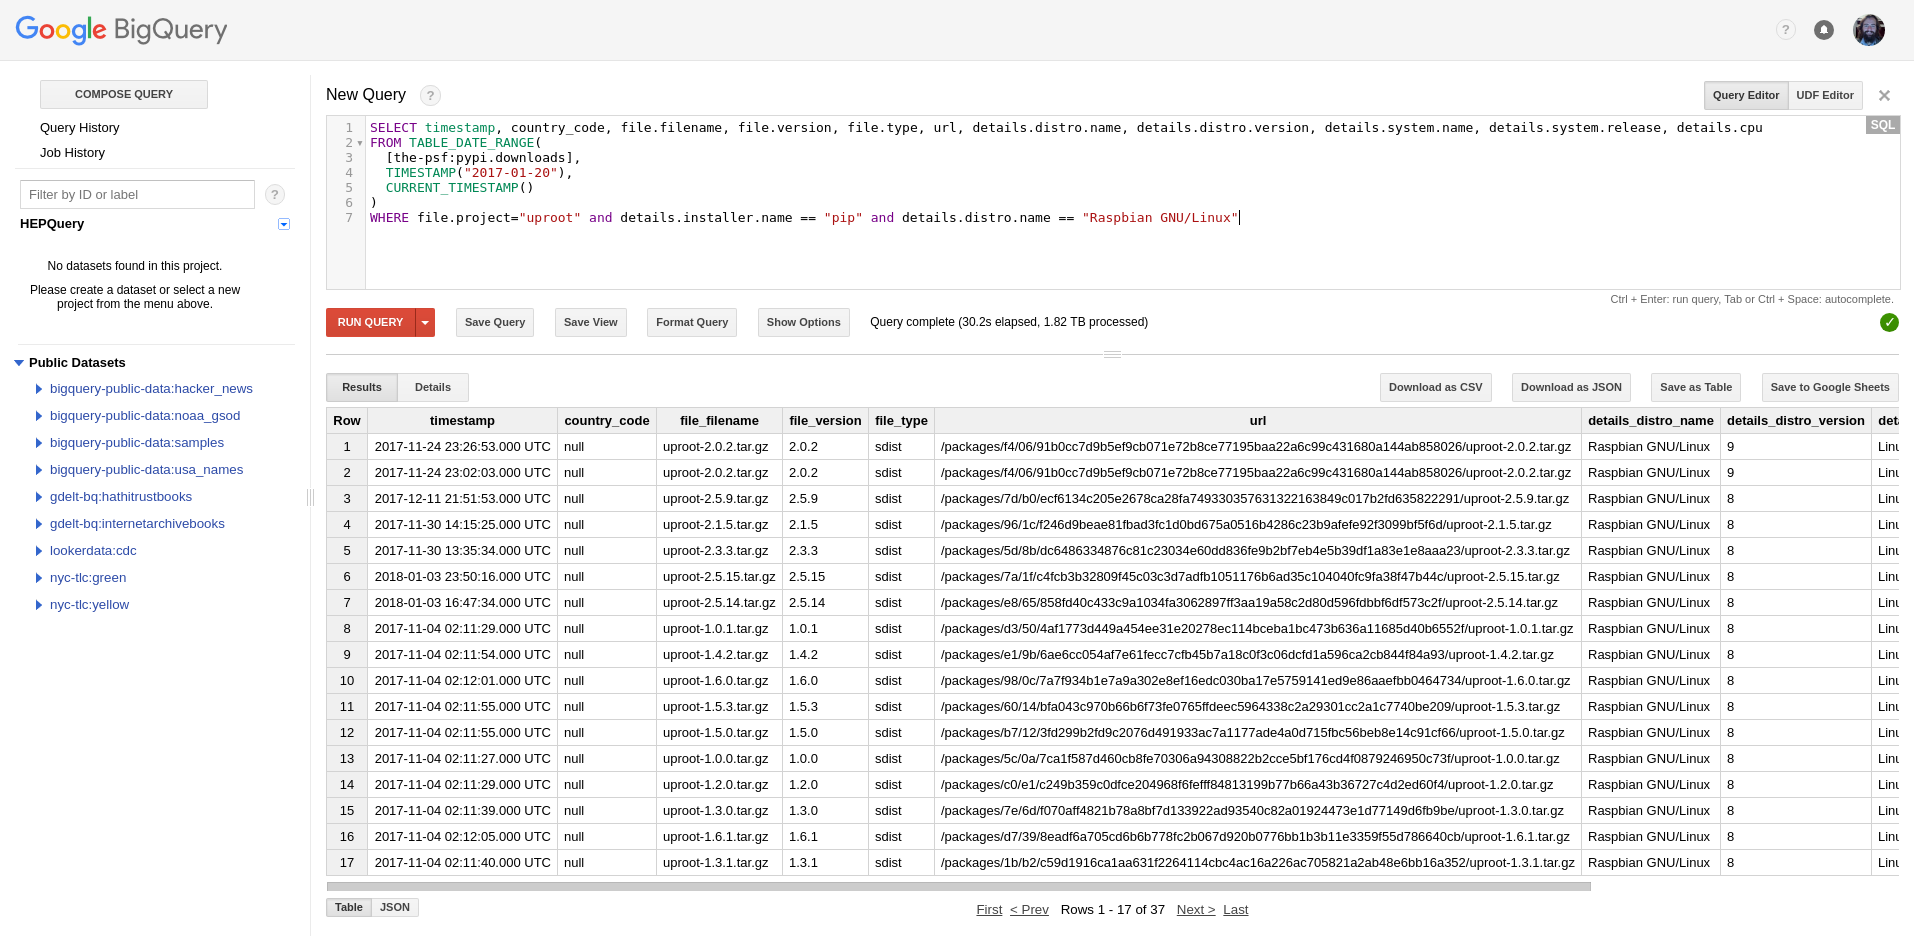
\includegraphics[width=\linewidth]{bigquery.png}
\end{columns}
\end{frame}

\begin{frame}{Basic block diagram}
\vspace{0.25 cm}
\begin{center}
\only<1-2>{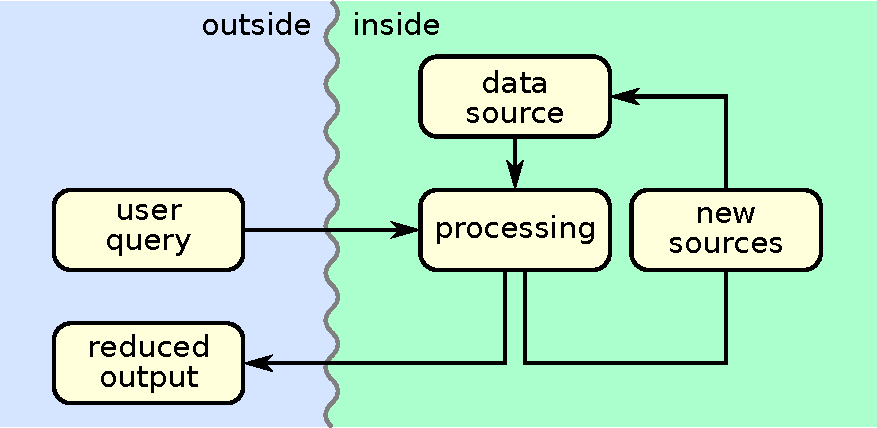
\includegraphics[width=0.7\linewidth]{basic-block-diagram.pdf}}
\only<3>{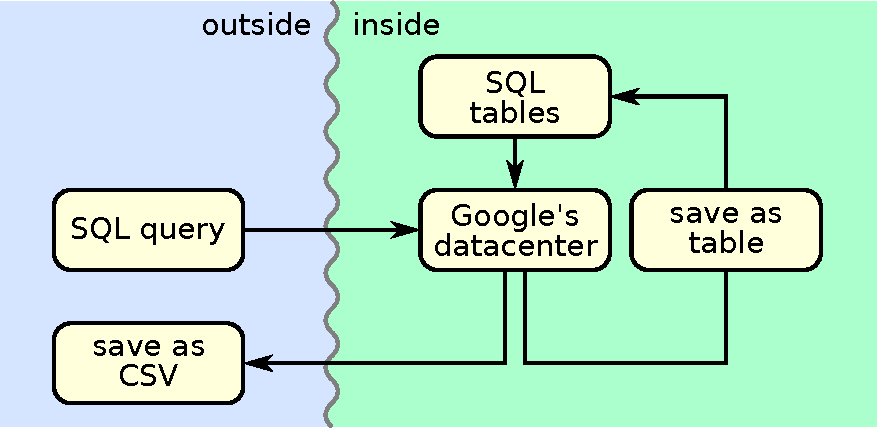
\includegraphics[width=0.7\linewidth]{google-block-diagram.pdf}}
\end{center}

\begin{uncoverenv}<2->
The ``new sources'' can be arbitrarily large and efficiently share overlapping data with the original sources because they live in the same system.

\vspace{0.25 cm}
The ``reduced output'' must be small enough to download quickly (e.g.\ histograms or highly skimmed tables). If not, the system ceases to be ``exploratory.''
\end{uncoverenv}
\end{frame}

\begin{frame}{So we can just use BigQuery, then?}
\vspace{0.25 cm}
\mbox{ } \hfill \textcolor{red}{\Huge No!!!} \hfill \mbox{ }

\vspace{0.1 cm}
\begin{itemize}\setlength{\itemsep}{0.2 cm}
\item<2-> \textcolor{darkblue}{Reason \#1: SQL.} Simple HEP problems translate into complex SQL and moderate-to-complex HEP problems would be unreasonably difficult to express.

\vspace{0.15 cm}
\textcolor{gray}{Non-SQL languages in this problem space, such as SparkSQL's column expressions or Apache Drill's internal query language, are just as restrictive in the ways that matter.}

\item<3-> \textcolor{darkblue}{Reason \#2: Data model.} The BigQuery paper (``Dremel''), Parquet \& Drill (open source versions of the same), Apache Arrow, and SparkSQL all describe rich, nested data models sufficient to describe HEP events.

\vspace{0.15 cm}
However, {\it for every one of these,} you quickly encounter ``not implemented yet'' messages when you try to use them for HEP events.

\item<4-> \textcolor{darkblue}{Reason \#3: User interface.} The web form is fun, but we need queries embedded in an interactive, programmable environment with plotting and statistics libraries: ROOT or Python or both (probably both).
\end{itemize}
\end{frame}

\begin{frame}{HEP is both simpler and more complex than SQL}
\vspace{0.35 cm}
\mbox{ } \hfill \textcolor{red}{\LARGE HEP data/functions are simpler} \hfill \mbox{ }

\vspace{0.25 cm}
\begin{columns}
\column{0.5\linewidth}

HEP functions never have to cross events.

\vspace{0.25 cm}
\mbox{ } \hfill 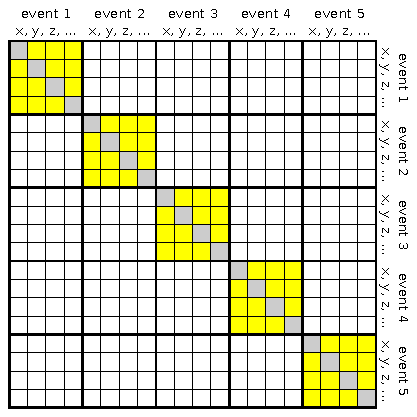
\includegraphics[width=0.8\linewidth]{event-variable-correlation-hep.pdf} \hfill \mbox{ }

\column{0.5\linewidth}

\mbox{\hspace{-0.5 cm}Common elsewhere: e.g.\ market basket analysis.\hspace{-0.5 cm}}

\vspace{0.25 cm}
\mbox{ } \hfill 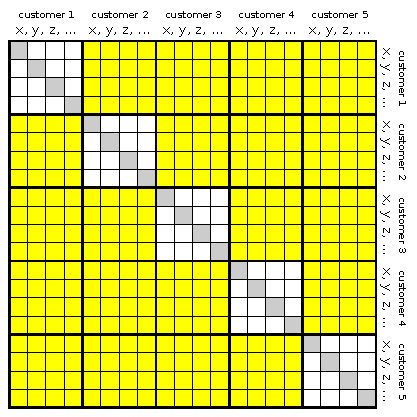
\includegraphics[width=0.8\linewidth]{event-variable-correlation-marketbasket-2.pdf} \hfill \mbox{ }

\end{columns}
\end{frame}

\begin{frame}{HEP is both simpler and more complex than SQL}
\vspace{0.35 cm}
\mbox{ } \hfill \textcolor{red}{\LARGE HEP data/functions are more complex} \hfill \mbox{ }

\vspace{-0.25 cm}
\begin{columns}[t]
\column{0.5\linewidth}

HEP data are variable-length, nested data structures, and we typically need to loop over combinations of particles.

\vspace{0.25 cm}
\mbox{ } \hfill 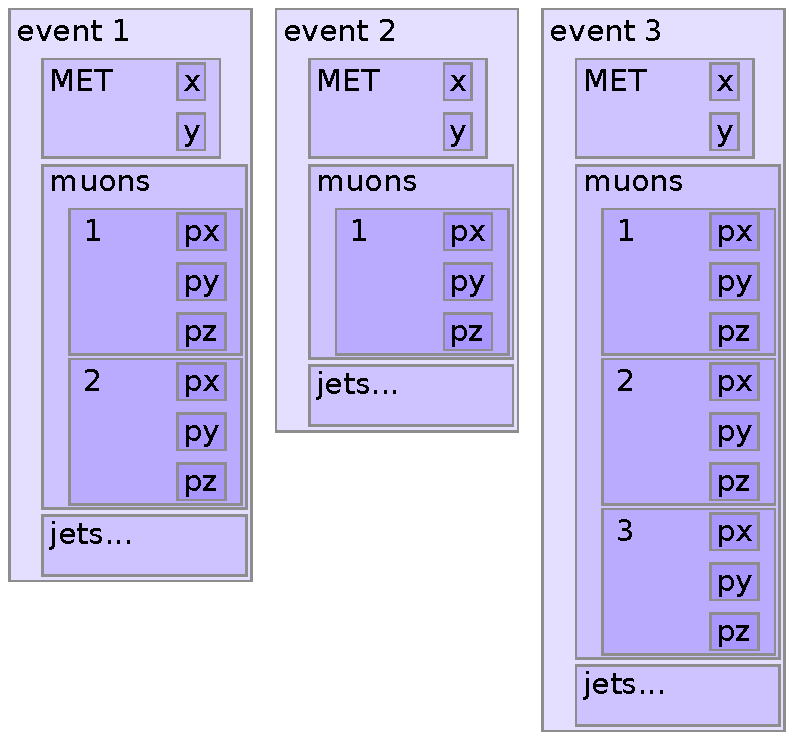
\includegraphics[width=0.8\linewidth]{event-structure.pdf} \hfill \hfill \mbox{ }

\column{0.5\linewidth}

In many fields, data are not considered ready for analysis until they're in a tabular form. (Earlier steps are called ``tidying.'')

\vspace{0.25 cm}
\mbox{ } \hfill 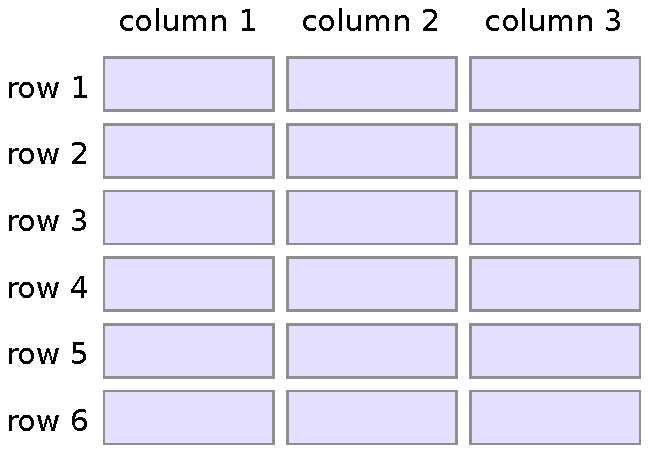
\includegraphics[width=0.8\linewidth]{table-structure.pdf} \hfill \hfill \mbox{ }

\end{columns}
\end{frame}

\begin{frame}{HEP is both simpler and more complex than SQL}
\Large
\renewcommand{\arraystretch}{2}
\mbox{\hspace{-0.35 cm}\begin{tabular}{c | c c}
                             & independent events & all-to-all shuffle \\\hline
tabular data                 & basic spreadsheet  & classic map-reduce \\
variable-length, nested data & \textcolor{red}{\underline{HEP analysis}} & graph analysis \\
\end{tabular}}
\end{frame}

\begin{frame}{What should our data source be?}
\vspace{0.5 cm}
\textcolor{darkblue}{Identically typed, variable-length, nested data can be split into columns:}
\begin{itemize}
\item All attribute values at a given level of hierarchy are stored together and may be retrieved independently of the rest.
\item Good for reading only the dozen interesting attributes.
\item ROOT has been doing this for years.
\end{itemize}

\begin{uncoverenv}<2->
\vspace{0.25 cm}
\textcolor{darkblue}{But beyond ROOT:}
\begin{itemize}
\item<2-> Want to adopt an optimization common in SQL: ``no row materialization.'' \\ User code written in terms of objects, but runtime is strictly array access (fast).
\item<3-> Want flexibility to define datasets with 99\% overlap: e.g.\ user defines new jet energy corrections for later use. New dataset is one new column + all old columns.
\item<4-> Want to allow for database-style indexing, so that a cut on an indexed variable (most likely $p_T$) avoids touching disk for events that would fail the cut.
\end{itemize}
\end{uncoverenv}
\end{frame}

\begin{frame}{Working implementation: OAMap}
\vspace{0.5 cm}
\underline{Object Array Map} (\href{https://github.com/diana-hep/oamap}{\textcolor{blue}{\tt https://github.com/diana-hep/oamap}})

\vspace{0.25 cm}
\begin{itemize}\setlength{\itemsep}{0.25 cm}
\item[$\surd$]<2-> Translates object oriented (Python) code into nothing but array operations.
\item[$\surd$]<3-> Extends Numba (Python compiler) to generate native machine bytecode (fast).
\item[$\surd$]<4-> Unrestricted source of arrays; may be ROOT, raw data files, remote network calls, HDF5, etc., or {\it all of the above in the same object.}
\item[$\surd$]<5-> Enough indirection for different particle types to be independently sorted by their own $p_T$s, and thus a filter like ``muon $p_T > X$ and jet $p_T > Y$'' might touch disk for only half the muon data and half the jet data (PoC).
\end{itemize}
\end{frame}

\begin{frame}[fragile]{OAMap example}
\small
\begin{minted}{python}
>>> import uproot
>>> import oamap.source.root

>>> url = "http://scikit-hep.org/uproot/examples/HZZ.root"
>>> events = uproot.open(url)["events"].oamap()
>>> events.schema.content["muons"].show()
List(
  starts = 'NMuon',    # schema maps object attributes to array names
  stops = 'NMuon',
  content = Record(    # at all levels of nesting
    fields = {
      'px': Primitive(dtype('float32'), data='Muon_Px'),
      'py': Primitive(dtype('float32'), data='Muon_Py'),
      'pz': Primitive(dtype('float32'), data='Muon_Pz'),
      'energy': Primitive(dtype('float32'), data='Muon_E'),
      'charge': Primitive(dtype('int32'), data='Muon_Charge'),
      'isolation': Primitive(dtype('float32'), data='Muon_Iso')
    }))
\end{minted}
\end{frame}

\begin{frame}[fragile]{OAMap example}
\vspace{0.5 cm}
\small
{\normalsize The dataset appears to be a nested Python list.}
\begin{minted}{python}
>>> events
[<Event at index 0>, <Event at index 1>, <Event at index 2>, ...,
 <Event at index 2418>, <Event at index 2419>, <Event at index 2420>]

>>> events[0].muons
[<Muon at index 0>, <Muon at index 1>]

>>> [x.px for x in events[0].muons]
[-52.899456, 37.73778]
\end{minted}

\vspace{0.5 cm}
{\normalsize But it is generated on demand from arrays.}
\begin{verbatim}
"NMuon":   array([2, 1, 2, ..., 1, 1, 1], dtype=int32)
"Muon_Px": array([-52.899456,  37.73778,  -0.81645936, ...,
                  -29.756786, 1.1418698,  23.913206  ], dtype=float32)
\end{verbatim}
\end{frame}

\begin{frame}[fragile]{OAMap example}
\vspace{0.5 cm}
\scriptsize
{\normalsize The dataset can be included in compiled code with no change in syntax.}
\begin{minted}{python}
>>> import numpy
>>> import numba
>>> import oamap.compiler
>>> @numba.njit                 # declares the following function to be compiled
... def compute(events, out):
...     i = 0
...     for event in events:    # "event" and "event.muons" are a compiler fiction
...         if len(event.muons) == 2:
...             mu1, mu2 = event.muons[0], event.muons[1]
...             px = mu1.px + mu2.px
...             py = mu1.py + mu2.py
...             pz = mu1.pz + mu2.pz
...             energy = mu1.energy + mu2.energy
...             out[i] = sqrt(energy**2 - px**2 - py**2 - pz**2)
...             i += 1

>>> out = numpy.empty(1371)
>>> compute(events, out)        # compilation and array-fetching happen on first call
>>> out
array([90.22780609, 74.74654388, 89.75765991, ..., 92.06494904,
       85.44384003, 75.96061707])
\end{minted}
\end{frame}

\begin{frame}{Current thinking\ldots}
\vspace{0.5 cm}
\begin{center}
\only<1>{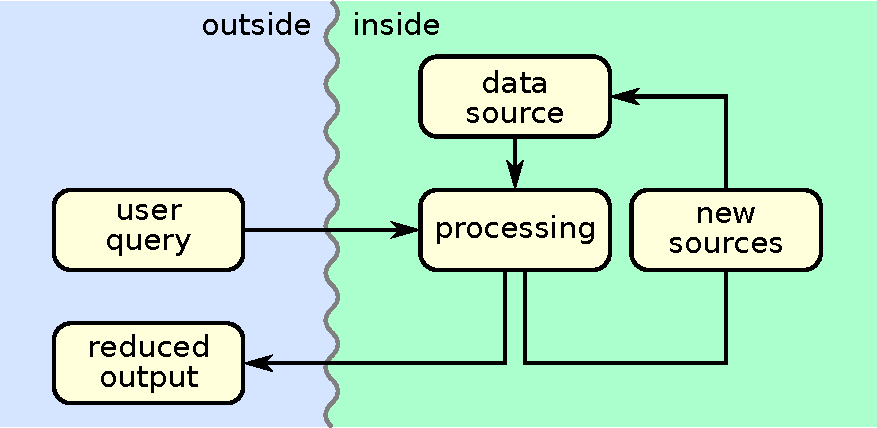
\includegraphics[width=0.7\linewidth]{basic-block-diagram.pdf}}
\only<2>{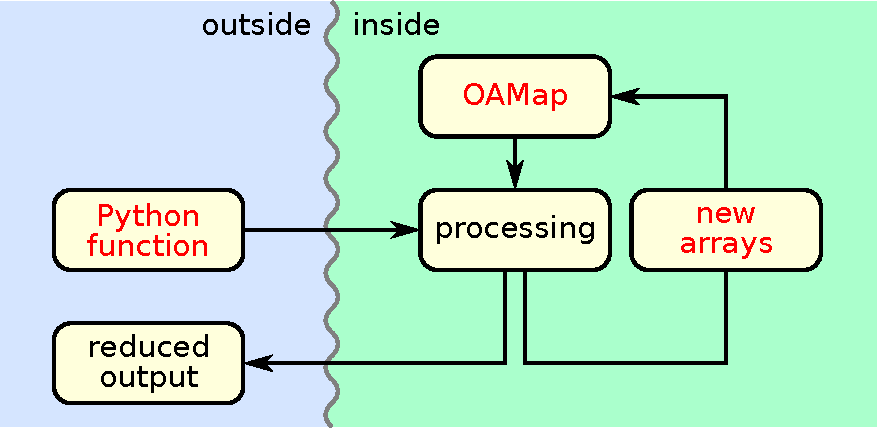
\includegraphics[width=0.7\linewidth]{block-diagram-source.pdf}}
\end{center}
\end{frame}

\begin{frame}{What should our reduced output be?}
\vspace{0.5 cm}
\textcolor{darkblue}{Simplest case:} histograms, but that would get restrictive as analyses develop.

\vspace{0.25 cm}
\uncover<2->{\textcolor{darkblue}{Here's an idea:} Pandas DataFrames.}

\vspace{0.5 cm}
\begin{itemize}\setlength{\itemsep}{0.25 cm}
\item<3-> Until recently, I've wrongly thought that a Pandas DataFrame is like a TTree with egregious limitations:
\begin{itemize}
\item Tabular, with little support for variable-length, nested data.
\item Strictly in-memory. \textcolor{gray}{(Dask DataFrames implement the interface \mbox{without this restriction.)\hspace{-1 cm}}}
\end{itemize}
\item<4-> I had been missing an important fact: most of Pandas's functionality is in its handling of {\it indexes}.
\begin{itemize}
\item TTrees/events are indexed only by entry or run/event number.
\item Pandas indexes may be non-contiguous, non-numeric, intervals/durations, multi-component, \ldots, and every operation maintains consistent indexes.
\end{itemize}
\item<5-> Pandas has more in common with {\it histograms} than it does with {\it event sources.}
\end{itemize}
\end{frame}

\begin{frame}{Just an example\ldots}
\vspace{0.25 cm}
\mbox{ } \hfill 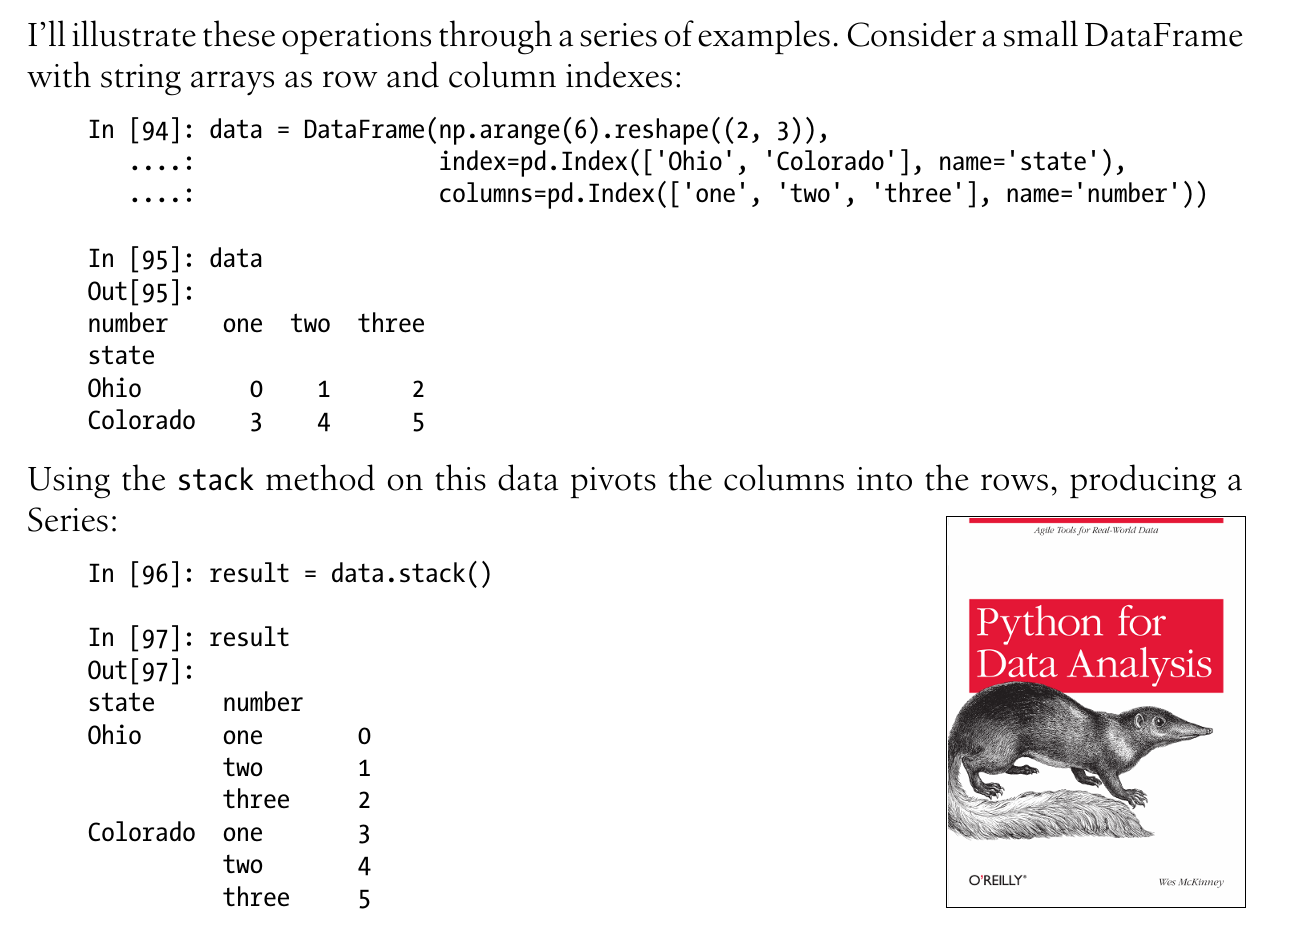
\includegraphics[width=0.78\linewidth]{pandas-book.png} \hfill \mbox{ }
\end{frame}

\begin{frame}[fragile]{Pandas generalizes what we do with histograms}
\small

\begin{minted}{python}
# define bins in many dimensions; we'll think about how to plot later
import pandhist
muonhist = (pandhist
            .bin(100, 0, 500, "mass")
            .cut("q1*q2 < 0")
            .irrbin([0.2, 0.5], "mt1")
            .irrbin([0.2, 0.5], "mt2")
            .fillable())      # creates a fillable Pandas DataFrame
\end{minted}

\begin{minted}{python}
for muons, charge, mt2activity in uproot.iterate(
  "RA2Analysis/*.root", "TreeMaker2/PreSelection",
  ["Muons", "Muons_charge", "Muons_MT2Activity"], outputtype=tuple):
    for i in range(len(muons)):
        if len(charge[i]) == 2:
            mu1, mu2 = muons[i]
            q1,  q2  = charge[i]
            mt1, mt2 = mt2activity[i]
            # fill method has an argument for each variable
            muonhist.fill((mu1 + mu2).mass, q1, q2, mt1, mt2)
\end{minted}
\end{frame}

\begin{frame}[fragile]{Pandas generalizes what we do with histograms}
\scriptsize
\begin{verbatim}
>>> muonhist
                                                  count   # in this example, count is
mass           q1*q2 < 0 mt1         mt2                  # the only column; the rest
[-inf, 0.0)    fail      [-inf, 0.2) [-inf, 0.2)    0.0   # is a hierarchical index
                                     [0.2, 0.5)     0.0   # (mass, q1*q2 < 0, mt1, mt2)
                                     [0.5, inf)     0.0
                         [0.2, 0.5)  [-inf, 0.2)    0.0
                                     [0.2, 0.5)     0.0   # if we asked for weights,
                                     [0.5, inf)     0.0   # sumw and sumw2 would be
                         [0.5, inf)  [-inf, 0.2)    0.0   # separate columns
                                     [0.2, 0.5)     0.0
                                     [0.5, inf)     0.0
               pass      [-inf, 0.2) [-inf, 0.2)    0.0   # if we asked for a profile,
                                     [0.2, 0.5)     0.0   # we'd get sum(y) and sum2(y)
                                     [0.5, inf)     0.0
                         [0.2, 0.5)  [-inf, 0.2)    0.0
                                     [0.2, 0.5)     0.0   # but most of the work is done
                                     [0.5, inf)     0.0   # by the hierarchical index
                         [0.5, inf)  [-inf, 0.2)    0.0
                                     [0.2, 0.5)     0.0
                                     [0.5, inf)     0.0
...                                                 ...
[1836 rows x 1 columns]
\end{verbatim}
\end{frame}

\begin{frame}[fragile]{Pandas generalizes what we do with histograms}
\small
\begin{onlyenv}<1>
\begin{minted}{python}
>>> pandhist.steps("mass").data(muonhist)
\end{minted}
\end{onlyenv}
\begin{onlyenv}<2>
\begin{minted}{python}
>>> pandhist.steps("mass").overlay("q1*q2 < 0").data(muonhist)
\end{minted}
\end{onlyenv}
\begin{onlyenv}<3>
\begin{minted}{python}
>>> pandhist.area("mass").stack("q1*q2 < 0").data(muonhist)
\end{minted}
\end{onlyenv}
\begin{onlyenv}<4>
\begin{minted}{python}
>>> pandhist.steps("mass").column("q1*q2 < 0").data(muonhist)
\end{minted}
\end{onlyenv}
\begin{onlyenv}<5>
\begin{minted}{python}
>>> pandhist.steps("mass").row("mt1").column("mt2").data(muonhist)
\end{minted}
\end{onlyenv}
\begin{onlyenv}<6>
\scriptsize
\begin{minted}{python}
>>> pandhist.steps("mass").overlay("q1*q2 < 0").row("mt1").column("mt2").data(muonhist)
\end{minted}
\end{onlyenv}

\begin{center}
\begin{onlyenv}<1>
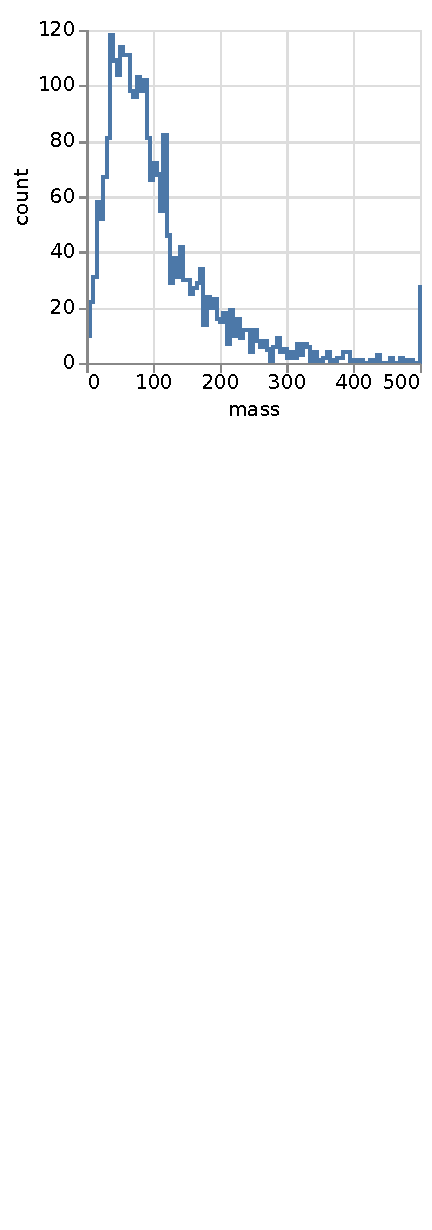
\includegraphics[height=7 cm]{pandhist.pdf}
\end{onlyenv}
\begin{onlyenv}<2>
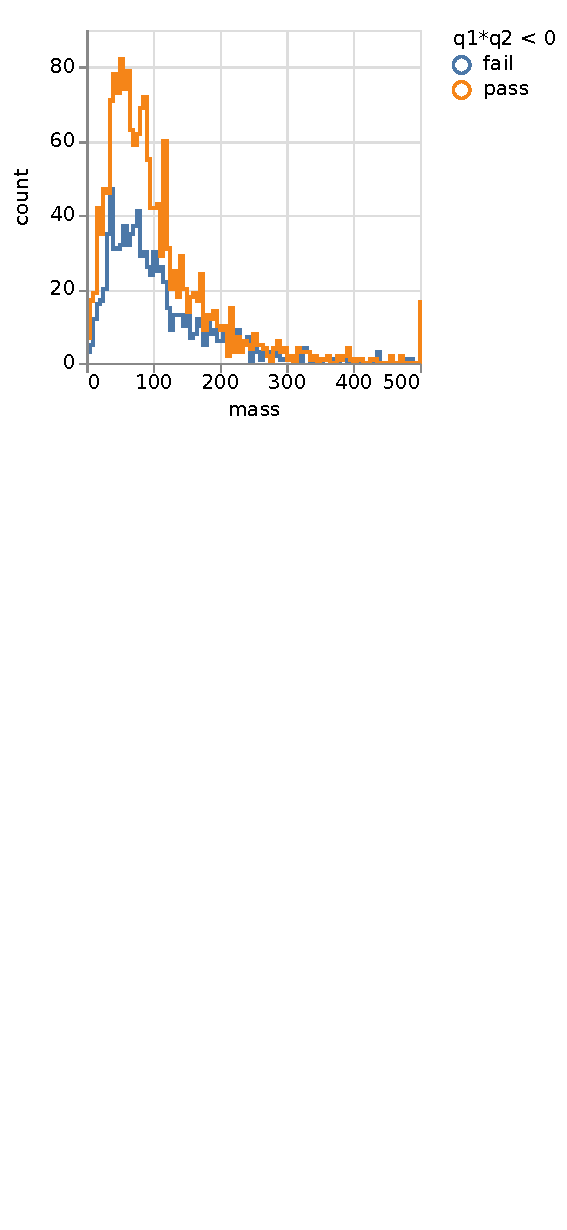
\includegraphics[height=7 cm]{pandhist_overlay.pdf}
\end{onlyenv}
\begin{onlyenv}<3>
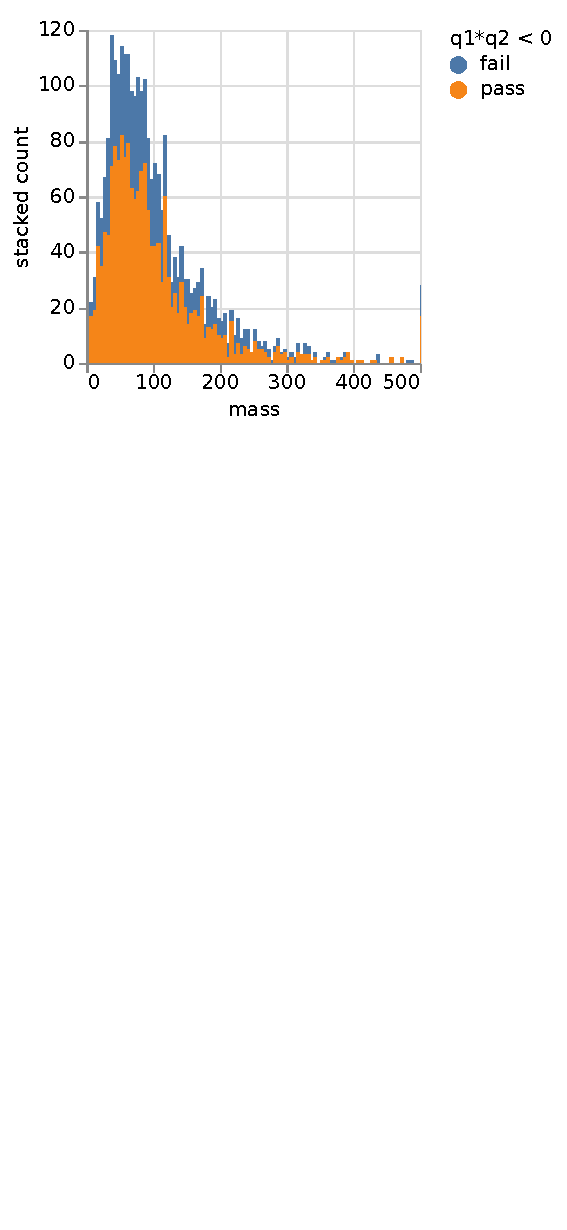
\includegraphics[height=7 cm]{pandhist_stack.pdf}
\end{onlyenv}
\begin{onlyenv}<4>
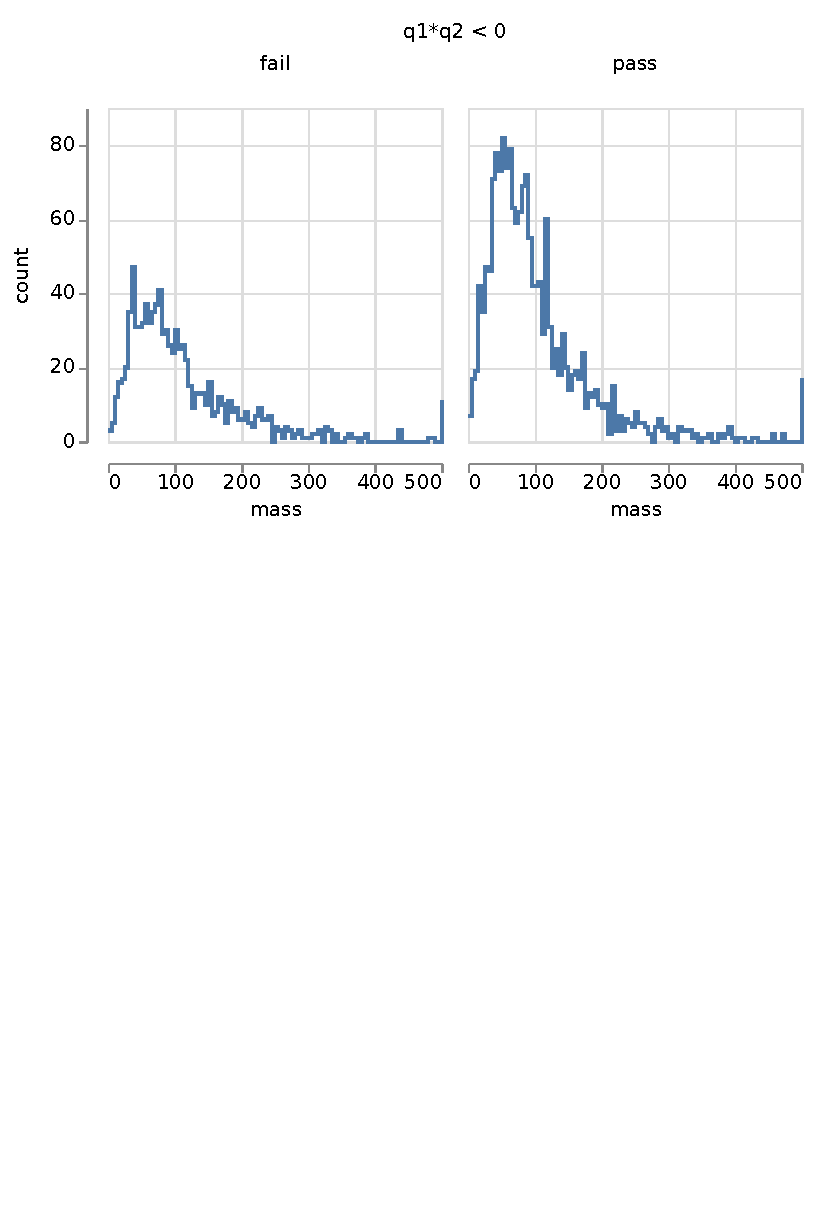
\includegraphics[height=7 cm]{pandhist_trellis.pdf}
\end{onlyenv}
\begin{onlyenv}<5>
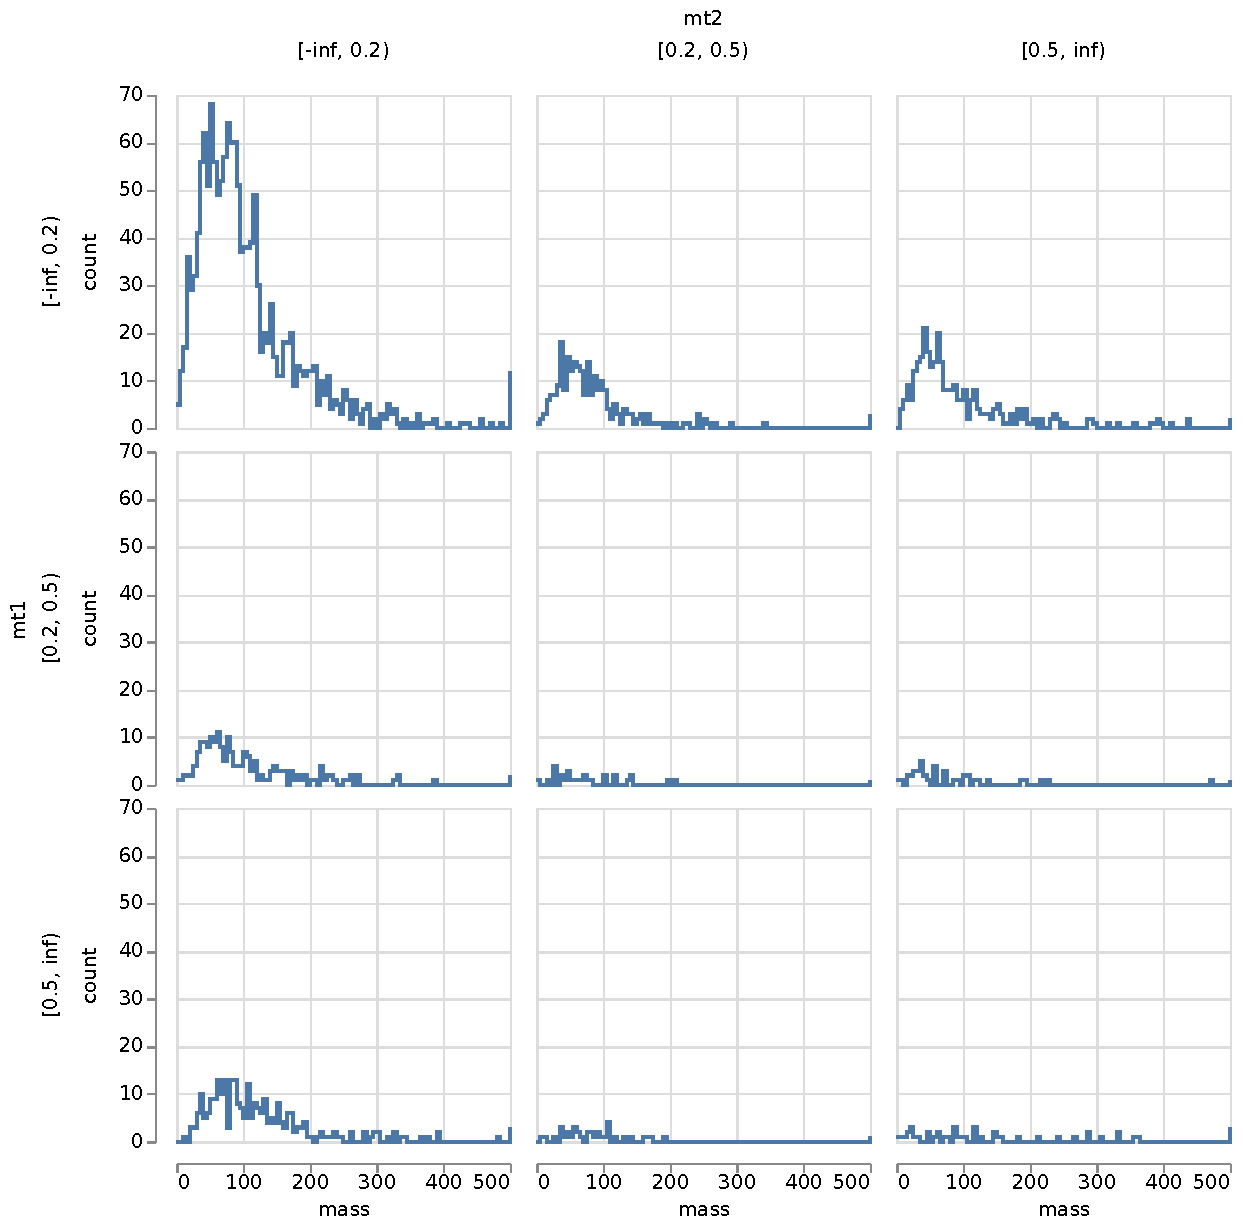
\includegraphics[height=7 cm]{pandhist_double_trellis.pdf}
\end{onlyenv}
\begin{onlyenv}<6>
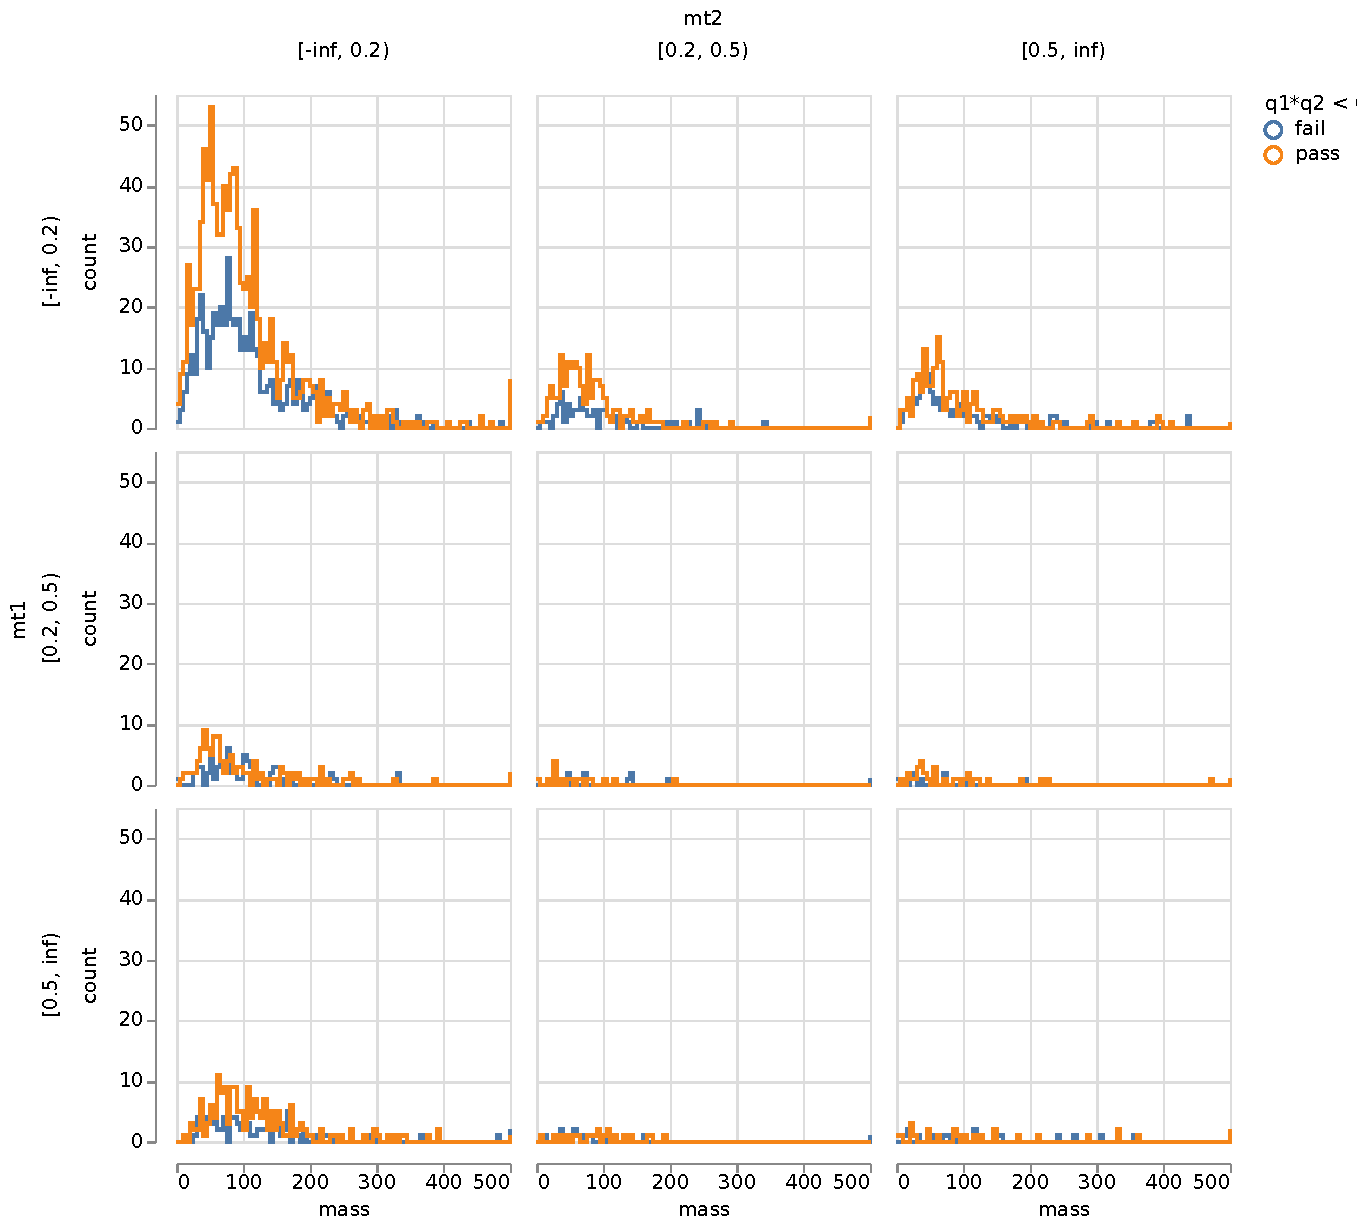
\includegraphics[height=7 cm]{pandhist_double_trellis_overlay.pdf}
\end{onlyenv}
\end{center}
\end{frame}

\begin{frame}{Current thinking\ldots}
\vspace{0.5 cm}
\begin{center}
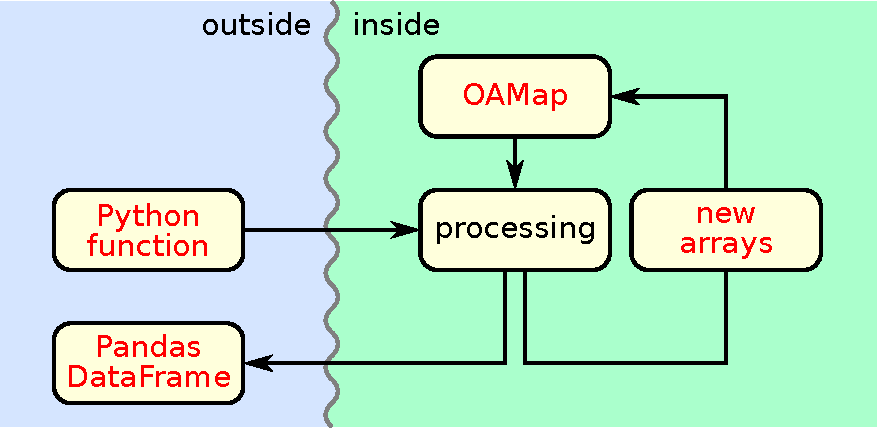
\includegraphics[width=0.7\linewidth]{block-diagram-output.pdf}
\end{center}
\end{frame}

\begin{frame}{What should our processing be?}
\vspace{0.5 cm}
\underline{Speedy, prompt start-up parallel processing is not something HEP needs to invent.}

\vspace{0.25 cm}
\begin{itemize}\setlength{\itemsep}{0.25 cm}
\item<2-> \textcolor{darkblue}{Spark} is the elephant in the room (used to be Hadoop), but it's hard to (efficiently) bridge our C++/Python ecosystem with the JVM.

\item<3-> I considered \textcolor{darkblue}{Drill}, but it's also JVM.

\item<4-> \textcolor{darkblue}{Impala} is C++, but seems to be too specialized to the SQL mindset.

\item<5-> Thanat Jatuphattharachat (summer student) investigated raw \textcolor{darkblue}{Zookeeper} coordination, but this is getting close to DIY.

\item<6-> \textcolor{darkblue}{Dask} looks like a good choice: it's in the C++/Python world, general enough to piece together what we need out of basic parts.

\vspace{0.25 cm}
(More about this in the concurrency session.)
\end{itemize}
\end{frame}

\begin{frame}{Current thinking\ldots}
\vspace{0.5 cm}
\begin{center}
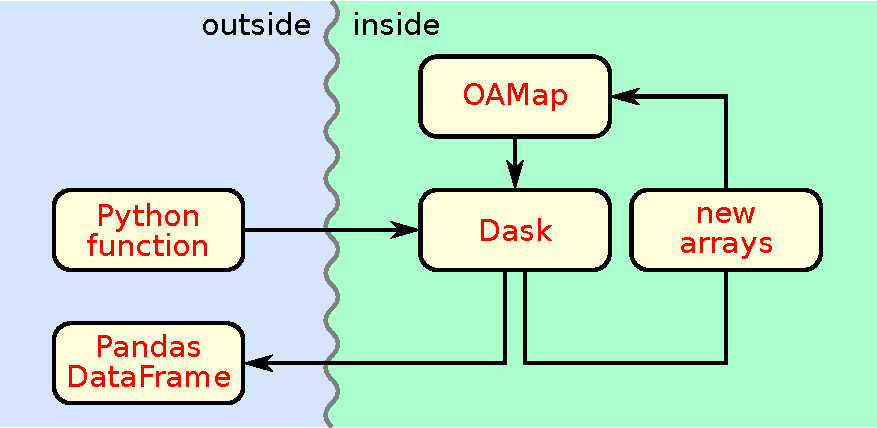
\includegraphics[width=0.7\linewidth]{block-diagram-processing.pdf}
\end{center}
\end{frame}

\begin{frame}{What should our data storage be?}
\vspace{0.5 cm}
\underline{Again, no need for HEP to invent.}

\vspace{0.25 cm}
\begin{itemize}\setlength{\itemsep}{0.25 cm}
\item<2-> Using columns, rather than files, as the fundamental unit means keeping track of a much larger number of named entities.

\item<3-> Object stores scale to larger namespaces than filesystems by providing fewer operations (listing, directory structure), which we don't need for this project.

\item<4-> \textcolor{darkblue}{Ceph} is both an object store and a filesystem, and it minimizes metadata overhead by coordinating data placement through a static function, rather than a dynamic service.

\begin{itemize}
\item<5-> Lets us experiment both ways.

\item<5-> We could use the static function to place executable tasks, improving data locality\ldots
\end{itemize}
\end{itemize}
\end{frame}

\begin{frame}{Current thinking\ldots}
\vspace{0.5 cm}
\begin{center}
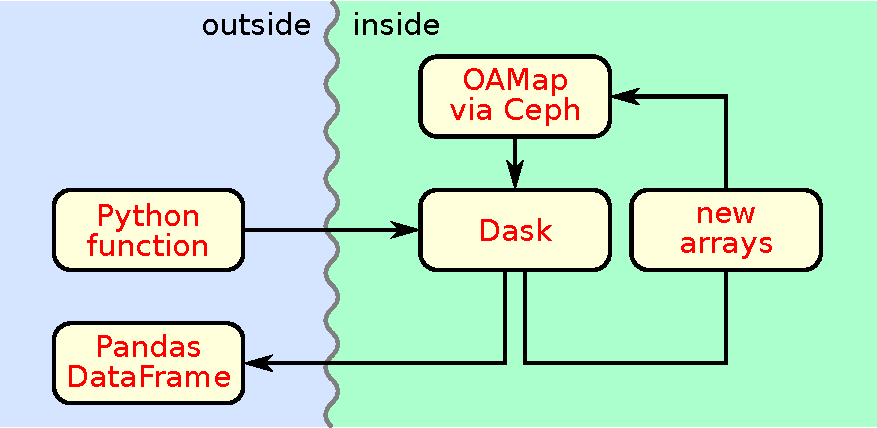
\includegraphics[width=0.7\linewidth]{block-diagram-ceph.pdf}
\end{center}
\end{frame}

\begin{frame}{Conclusions}
\vspace{0.35 cm}
Though an analysis service should use as many off-the-shelf parts as possible, some are not suitable and some essential functionality is nonexistent.

\vspace{0.25 cm}
\underline{Software products developed along the way:}

\renewcommand{\arraystretch}{1.2}

\vspace{0.25 cm}
\begin{tabular}{c p{0.65\linewidth} c}
\href{https://github.com/scikit-hep/uproot}{\textcolor{blue}{uproot}} & Quickly access ROOT branches as arrays. & mature \\
\href{https://github.com/diana-hep/oamap}{\textcolor{blue}{oamap}} & Translate between object oriented Python and low-level array operations. & beta \\
pandhist & Methods for plotting tables of intervals and counts as histograms (Vega for plotting). & experimental \\
vegascope & Browser-based TCanvas for Vega, so that you don't have to use Jupyter if you don't want to. & done \\
? & OAMap as a collection in Dask. & \\
? & Column and dataset manager (for sharing data). & \\
? & All-in-one environment for query-based analysis. & \\
\end{tabular}
\end{frame}

\end{document}
